\documentclass[]{book}
\usepackage{lmodern}
\usepackage{amssymb,amsmath}
\usepackage{ifxetex,ifluatex}
\usepackage{fixltx2e} % provides \textsubscript
\ifnum 0\ifxetex 1\fi\ifluatex 1\fi=0 % if pdftex
  \usepackage[T1]{fontenc}
  \usepackage[utf8]{inputenc}
\else % if luatex or xelatex
  \ifxetex
    \usepackage{mathspec}
  \else
    \usepackage{fontspec}
  \fi
  \defaultfontfeatures{Ligatures=TeX,Scale=MatchLowercase}
\fi
% use upquote if available, for straight quotes in verbatim environments
\IfFileExists{upquote.sty}{\usepackage{upquote}}{}
% use microtype if available
\IfFileExists{microtype.sty}{%
\usepackage{microtype}
\UseMicrotypeSet[protrusion]{basicmath} % disable protrusion for tt fonts
}{}
\usepackage[margin=0.5in]{geometry}
\usepackage{hyperref}
\hypersetup{unicode=true,
            pdftitle={UIL Enrollment Analysis},
            pdfauthor={Cary W. Reams},
            pdfborder={0 0 0},
            breaklinks=true}
\urlstyle{same}  % don't use monospace font for urls
\usepackage{natbib}
\bibliographystyle{apalike}
\usepackage{longtable,booktabs}
\usepackage{graphicx,grffile}
\makeatletter
\def\maxwidth{\ifdim\Gin@nat@width>\linewidth\linewidth\else\Gin@nat@width\fi}
\def\maxheight{\ifdim\Gin@nat@height>\textheight\textheight\else\Gin@nat@height\fi}
\makeatother
% Scale images if necessary, so that they will not overflow the page
% margins by default, and it is still possible to overwrite the defaults
% using explicit options in \includegraphics[width, height, ...]{}
\setkeys{Gin}{width=\maxwidth,height=\maxheight,keepaspectratio}
\IfFileExists{parskip.sty}{%
\usepackage{parskip}
}{% else
\setlength{\parindent}{0pt}
\setlength{\parskip}{6pt plus 2pt minus 1pt}
}
\setlength{\emergencystretch}{3em}  % prevent overfull lines
\providecommand{\tightlist}{%
  \setlength{\itemsep}{0pt}\setlength{\parskip}{0pt}}
\setcounter{secnumdepth}{5}
% Redefines (sub)paragraphs to behave more like sections
\ifx\paragraph\undefined\else
\let\oldparagraph\paragraph
\renewcommand{\paragraph}[1]{\oldparagraph{#1}\mbox{}}
\fi
\ifx\subparagraph\undefined\else
\let\oldsubparagraph\subparagraph
\renewcommand{\subparagraph}[1]{\oldsubparagraph{#1}\mbox{}}
\fi

%%% Use protect on footnotes to avoid problems with footnotes in titles
\let\rmarkdownfootnote\footnote%
\def\footnote{\protect\rmarkdownfootnote}

%%% Change title format to be more compact
\usepackage{titling}

% Create subtitle command for use in maketitle
\providecommand{\subtitle}[1]{
  \posttitle{
    \begin{center}\large#1\end{center}
    }
}

\setlength{\droptitle}{-2em}

  \title{UIL Enrollment Analysis}
    \pretitle{\vspace{\droptitle}\centering\huge}
  \posttitle{\par}
    \author{Cary W. Reams}
    \preauthor{\centering\large\emph}
  \postauthor{\par}
      \predate{\centering\large\emph}
  \postdate{\par}
    \date{2019-11-15}

\usepackage{booktabs}
\usepackage{amsthm}
\makeatletter
\def\thm@space@setup{%
  \thm@preskip=8pt plus 2pt minus 4pt
  \thm@postskip=\thm@preskip
}
\makeatother

\begin{document}
\maketitle

{
\setcounter{tocdepth}{1}
\tableofcontents
}
\chapter{Purpose}\label{purpose}

This has been created to explore R, bookdown, pandoc, tidyverse, etc.

\chapter{UIL}\label{uil}

Every two years, the governing body for public secondary school sports
uses attendance figures to create the classifications and districts of
competition for the schools in the state of Texas. This year's
announcement may be found on their site,
\href{http://www.uiltexas.org/athletics/conference-cutoffs}{here}. The
PDF file that was used to source the data is linked to from the same
page. Looks like a footnote at the bottom of the page.

Wanting to experiment more with R, the publication of enrollment figures
offers a nice large dataset (\textgreater{} 1400 entries) to use as a
training ground. R offers some of its own canned sets, but I work better
when I have some personal context for the data. In this case, Texas High
School Football (\texttt{\#txhsfb}).

\section{Data Source and Prep}\label{data-source-and-prep}

\begin{itemize}
\tightlist
\item
  Obtained original report from Texas UIL, as a PDF
\item
  Used \texttt{pstotext} to convert the PDF to PS then to an ASCII TXT
\item
  basic editor allowed for formatting the resulting file as a CSV using
  the pipe symbol rather than spaces or commas as field separators
\item
  slurped the CSV with a spreadsheet, manually corrected any remaining
  column disparities, then saved as CSV for R
\end{itemize}

\section{Pass One, All Schools}\label{pass-one-all-schools}

I dumped everything from the CSV file into an R boxplot request and got
this for my effort:

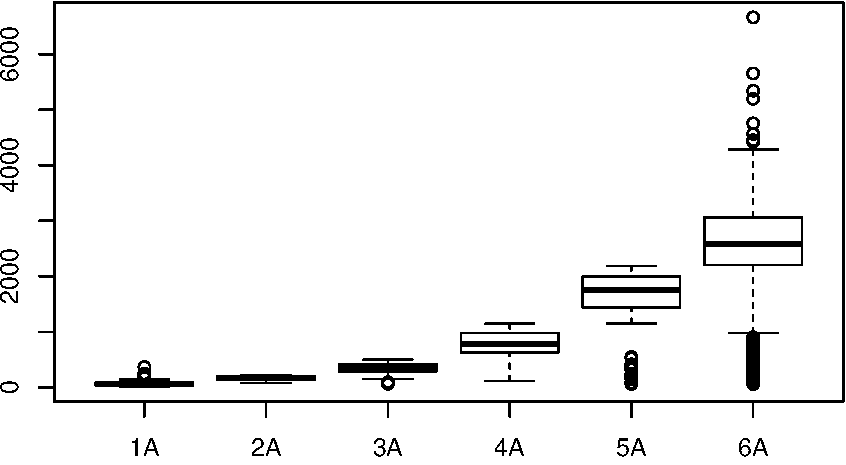
\includegraphics{texas-uil_files/figure-latex/unnamed-chunk-2-1.pdf}

You'll notice there are some significant outliers visible in the 6A
classification. That told me there were schools with really small
enrollments that were in the 6A classification. It didn't make any
sense. There must be a mistake.

There was. None of those schools play football.

So my second pass considered only schools that played football - that is
after all, my real interest here.

\section{Pass Two, Football-Playing
Schools}\label{pass-two-football-playing-schools}

Okay, so now things look different:

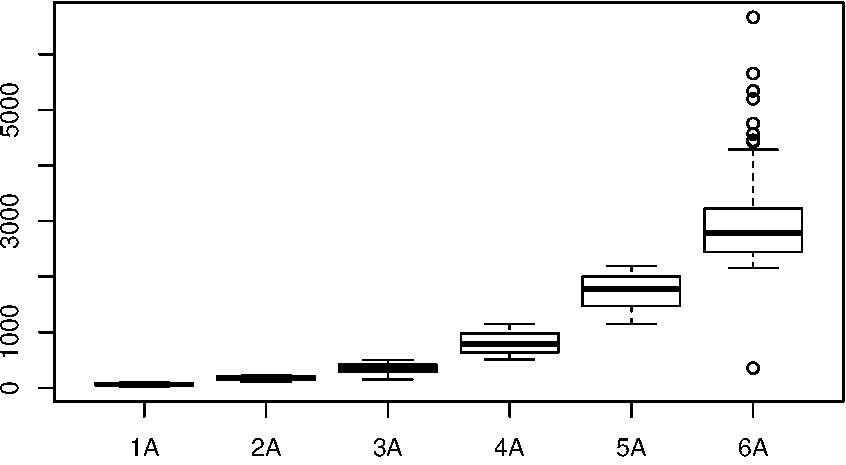
\includegraphics{texas-uil_files/figure-latex/unnamed-chunk-3-1.pdf}

But we still have an outlier. There's a school in 6A with an enrollment
of less than 500 ? Yep, lets find it.
\texttt{grep\ -n\ 6A\ football.csv\ \textbar{}\ grep\ -e\ \textquotesingle{}\textbar{}{[}0-9{]}\textbackslash{}\{3\textbackslash{}\}\textbar{}\textquotesingle{}}
yielded:

2:Fort Worth ISD \textbar{} FW Young Mens Leadership Acad \textbar{} 6A
\textbar{} x \textbar{} 11 Man \textbar{}354\textbar{}2018\\

And so I tried to find out if that was legitimate or some kind of typo.
It's not. Apparently this is a school that falls under a Texas UIL
requirement that forces it to play in the same classification as the
largest school in its governing school district. Since that's the Ft
Worth ISD, \ldots{} 6A it is.

\section{Distribution of Football-Playing
Schools}\label{distribution-of-football-playing-schools}

Finally, I wanted to look at the distribution of school sizes. It was
enlightening. Texas is a big, wide-spread state. There are only four
major population centers - Houston, Dallas / Ft. Worth, Austin, and San
Antonio.

Take a look at the enrollment distributions - bars represent increments
of 100 students.

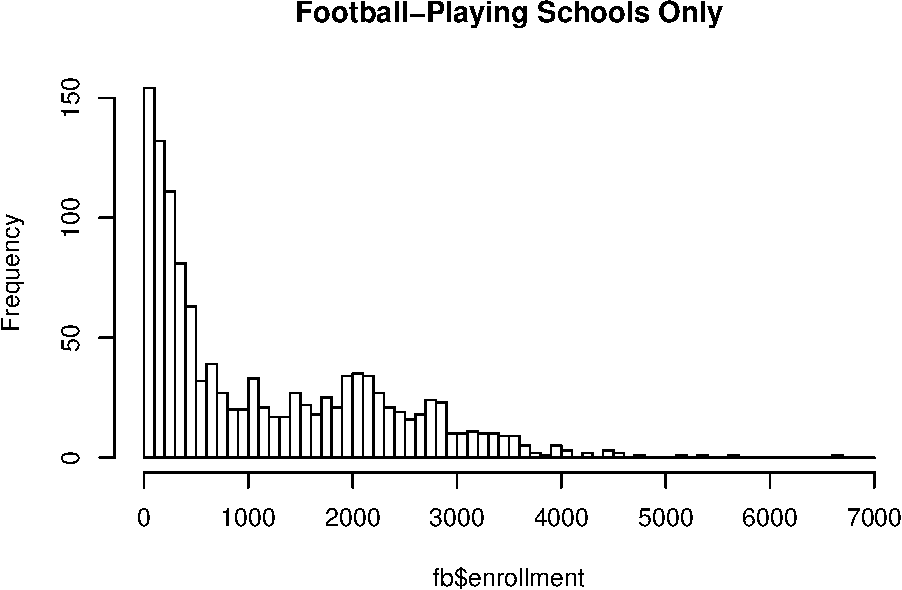
\includegraphics{texas-uil_files/figure-latex/unnamed-chunk-4-1.pdf}

\begin{center}\rule{0.5\linewidth}{\linethickness}\end{center}

raw data for this site may be found in the texas-hs-enrollment-analysis
directory of the repo for this github pages site

\bibliography{book.bib,packages.bib}


\end{document}
